\documentclass[11pt,border=4pt]{standalone}
\usepackage{amsmath,amssymb,bm,mathtools}
\usepackage[fontset=fandol]{ctex}
\usepackage{tikz}
\usetikzlibrary{arrows.meta,calc,patterns,angles,quotes,decorations.markings,decorations.pathmorphing}
\newcommand{\dd}{\mathop{}\!\mathrm d}
\newcommand{\e}{\mathrm e}
\tikzset{axis/.style={->,>=Stealth,line width=.45pt},world/.style={line width=.8pt},flow/.style={->,>=Stealth,line width=.7pt},ray/.style={->,>=Stealth,line width=.7pt},guide/.style={dashed,line width=.35pt},aux/.style={dashed,line width=.35pt},dim/.style={<->,>=Stealth,line width=.35pt},every node/.style={font=\small},force/.style={->,>=Stealth,very thick},gas/.style={fill=blue!7}}
\begin{document}
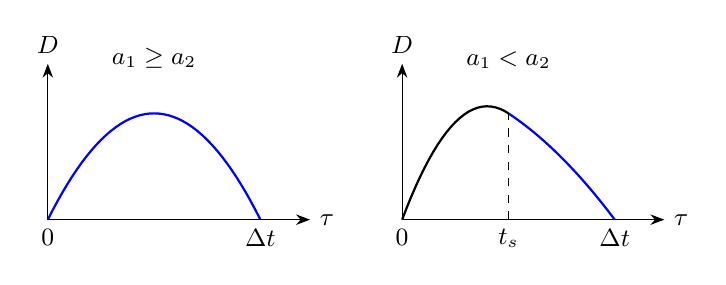
\begin{tikzpicture}[scale=.9]
\begin{scope}
\draw[axis](0,0)--(3.7,0)node[right]{$\tau$};\draw[axis](0,0)--(0,2.2)node[above]{$D$};
\draw[blue,world]plot[domain=0:1,samples=45]({3*\x},{6*\x*(1-\x)});
\node[below]at(0,0){$0$};\node[below]at(3,0){$\Delta t$};\node[above]at(1.5,2){$a_1\ge a_2$};
\end{scope}
\begin{scope}[xshift=5cm]
\draw[axis](0,0)--(3.7,0)node[right]{$\tau$};\draw[axis](0,0)--(0,2.2)node[above]{$D$};
\draw[world]plot[domain=0:.5,samples=25]({3*\x},{8*\x-10*(\x)^2});
\draw[blue,world]plot[domain=.5:1,samples=30]({3*\x},{2*(1-(\x)^2)});
\draw[guide](1.5,0)--(1.5,1.5);\node[below]at(0,0){$0$};\node[below]at(1.5,0){$t_s$};\node[below]at(3,0){$\Delta t$};\node[above]at(1.5,2){$a_1<a_2$};
\end{scope}
\end{tikzpicture}
\end{document}
